%Review of existing harmonic excitation.
%	Nonlinear Systems
%		Traditional Metrics (THD, IMD)
%		Minimisation of Nonlinear Distortion
%		Advent of "Nonlinear Niceness"
%	Timbre of nonlinear distortions (Martens and Marui type shit)
%	Uses of Harmonic Excitation
%	Harmonic Generation Methods
%		Static Nonlinearities
%		Bandwidth Extension (high frequency reconstruction)
%		Individual Harmonic Generation (SMC paper)
%		Psychoacoustic Enhancers

\chapter{Harmonic Excitation for Timbral Control}
\label{chap:ExcitationEvaluation}
	Harmonic excitation algorithms developed for the applications discussed in the Section \ref{sec:Excitation-Uses} are
	specialised to perform a particular task. As this work is concerned with the application of harmonic excitation to
	real time timbral control some algorithms in the literature may not be applicable. In Section
	\ref{sec:ExcitationEvaluation-Evaluation} a set of criteria for assessing the suitability of a harmonic excitation
	algorithms for use in this work are suggested. These criteria are then used to asses various algorithms in Section
	\ref{sec:ExcitationEvaluation-Comparison}, a summary of each algorithms performance shown in Table
	\ref{tab:ComparisonSummary}. Techniques for improving the performance of algorithms with respect to these criteria
	are discussed where appropriate.

\note
{
	Cite \citet{esqueda2015aliasing} about reducing aliasing in clippers.
}

\section{Evaluating Harmonic Excitation Algorithms for Use in Timbral Control}
\label{sec:ExcitationEvaluation-Evaluation}
	To prove useful for real time timbral control a harmonic excitation algorithm should provide efficient, intuitive
	control over where energy is introduced into a signal's spectrum. \citet{larsen2004audio} evaluate a number of
	algorithms for their use in bandwidth extension applications, discussing the spectral and temporal characteristics
	of the systems. Similar properties are required of algorithms used for real time timbral control which will be
	assessed again the following criteria:

	\begin{itemize}
		\item Complexity
		\item Homogeneity
		\item Spectral Characteristics
		\item Temporal Characteristics
		\item Flexibility
%		\item Naturalness.
	\end{itemize}

	The ideal characteristics within these areas are discussed in Sections
	\ref{sec:ExcitationEvaluation-Evaluation-Complexity} to \ref{sec:ExcitationEvaluation-Evaluation-Flexibility}.

	\subsection{Complexity}
	\label{sec:ExcitationEvaluation-Evaluation-Complexity}
		Audio effects can operate either offline or in real time. An offline effect is provided with a prerecorded
		input signal and processes it, taking as much time as is necessary. A real time effect processes an input
		signal in a short enough time that the output can be produced at the same rate at which the input is being
		provided. Real time processing speeds up music production as effect parameters can be adjusted while audio
		is playing and the results heard immediately. In order to achieve this the algorithms used in the effect
		must be efficient and operate with minimal latency. 

		In order to ease the computational load on the processor, digital audio processing if often done in blocks.
		A certain number of samples are recorded into a memory buffer and then all processed at once. This
		introduces some latency into the system; the processing buffer must be filled with samples from the input
		before an output can be produced. The larger the processing buffer size the more latency but the less the
		computational load as the cost of constructing and moving buffers is amortised across a greater number of
		samples. Any processing applied to the block of audio must be completed within the allowed latency time, if
		not there will be gaps between blocks during playback causing audible anomalies. For real time audio effects
		it is crucial to keep throughput latency to a minimum. \citet{lester2007the} suggest that, depending on the
		scenario, latencies as small as 1.4ms could be deemed unacceptable. In order to keep latency to a minimum,
		processing algorithms should be able to operate in real time when using a small buffer size. In a modern
		music production setting there may be several audio effects operating concurrently, the algorithms used for
		real time harmonic excitation must not only be efficient enough to run in real time but also to allow any
		concurrent processing to proceed uninterrupted.

		Occasionally it is necessary to introduce a specific amount delay as part of the processing algorithm, such
		as when applying a non-causal filter. This delay contributes to the overall latency of the effect and as
		such will be discussed alongside an algorithm's complexity.

	\subsection{Homogeneity}
	\label{sec:ExcitationEvaluation-Evaluation-Homogeneity}
		To make the application of an audio effect more intuitive it should produce similar perceived timbral
		manipulations for all input signals. Often this is not the case with traditional audio signal processing
		methods. For example, an equaliser can be used to amplify a certain band of frequencies is a signal. The
		spectra of signals with energy in this frequency range will be altered while those of signals with no energy
		in that band will be unaffected. This problem is compounded when the effect being applied is non-homogeneous
		(does not satisfy the condition of homogeneity given by Equation \ref{eq:homogeneity}). Nonlinear systems
		are typically non-homogeneous, this is undesirable when using them to achieve timbral control as it means
		the effects are less easy to predict. A non-homogeneous system behaves differently depending on the
		amplitude of the input signal. Different timbral transforms could be applied to the same signal if
		its amplitude is changed slightly. From a user's point of view this makes control of the system less
		intuitive as the perceived function of control parameters can change depending on signal level. The
		algorithms used in harmonic excitation systems for timbral control should exhibit homogeneous behaviour in
		order to increase the systems intuitiveness.

	\subsection{Spectral Characteristics}
	\label{sec:ExcitationEvaluation-Evaluation-SpectralCharacteristics}
		The algorithms presented in Section \ref{sec:Excitation-Methods} all introduce new spectral content to a
		signal. Depending on the algorithm and the input signal the nature of this this new content can vary
		greatly, ranging from wide bands comprising both harmonic and inharmonic partials to an individual harmonic
		partial. To provide intuitive timbral control it is desirable that these spectral effects can be controlled
		reliably for a wide range of input signals. An ideal algorithm would allow for control over the position,
		width and content of the band of energy introduced. For example a system designed to only generate harmonic
		partials should not introduce inharmonicity for any input signal. The system must be configured such that
		none of the distortion components will lie at inharmonic frequencies and a limit should be set on the
		maximum frequency generated to avoid aliasing being a potential source of inharmonicity.

	\subsection{Temporal Characteristics}
	\label{sec:ExcitationEvaluation-Evaluation-TemporalCharacteristics}		
		\citet{larsen2004audio} discuss the temporal effects of several bandwidth extension algorithms. Their
		primary concern however is ensuring that as little alteration is made to the temporal properties of a
		signal's amplitude envelope as possible. For timbral manipulation it is not necessary to be this
		restrictive, systems which change a signal's temporal properties may prove useful for controlling certain
		aspects of timbre. As with a system's spectral characteristics the temporal characteristics of a system used
		to timbral control should be predictable and similar across a large range of input signals.

	\subsection{Flexibility}
	\label{sec:ExcitationEvaluation-Evaluation-Flexibility}
		Different timbral transformations may require vastly different processing to be applied to the signal. The
		flexibility of a harmonic excitation algorithm refers to its ability to be used for a number of different
		audio processing tasks. A highly flexibly algorithm will provide a large degree of control over its spectral
		and temporal characteristics, thereby allowing a user to achieve their desired timbral effect. Users with no
		knowledge of how a particular harmonic excitation system is constructed will have difficulty setting its
		parameters to achieve this effect. To combat this, abstracted semantic parameters can be devised which alter
		the relevant parameters of the underlying harmonic excitation system. The flexibility of an algorithm also
		takes into account how easily its parameters can be mapped to semantic control parameters. For example, a
		system which proved parameters for the amplitudes of individual harmonics in the output is more flexible as
		it can be used for generating both large bands of spectral energy but also in situations where fine control
		of the spectral structure is required. 

		As in many fields a balance between flexibility and ease of use must be made when deciding which technique
		to use. If the system is overly generalised it may require a large amount of work to achieve a simple task.
		In the discussion of the flexibility of each harmonic excitation algorithm (Section
		\ref{sec:ExcitationEvaluation-Comparison-Flexibility}) the control provided over how they alters the
		properties of an input signal will be discussed along with processing applications they may be useful for.

\section{Method Comparison}
\label{sec:ExcitationEvaluation-Comparison}
	In this section the algorithms discussed in Section \ref{sec:Excitation-Methods} are evaluated against the criteria
	given in Section \ref{sec:ExcitationEvaluation-Evaluation}. For each criteria the relevant characteristics of each
	algorithm are discussed in Sections \ref{sec:ExcitationEvaluation-Comparison-Complexity} to
	\ref{sec:ExcitationEvaluation-Comparison-Flexibility}. Where appropriate techniques for improving the performance of
	an algorithm in a particular area are suggested and discussed. A summary of each of the algorithm's performance in
	each area is given in Table \ref{tab:ComparisonSummary}.

	\begin{landscape}
	\subsection{Comparison Summary}
	\label{sec:ExcitationEvaluation-Comparison-Summary}
		\begin{table}[h!]
			\centering
			\begin{tabular}{|c|c|C{4cm}|C{5cm}|C{5cm}|}
				\hline
				\bf{Method} & \bf{Complexity} & \bf{Homogeneity} & \bf{Spectral Characteristics} & 
				\bf{Temporal Characteristics} \tabularnewline 
				% & \bf{Naturalness}
				\hline
				\hline
				Static Nonlinearity & $\mathcal{O}(n)$ & Non-homogeneous &
				Order (odd /  even) and roll off, can be bandlimited & 
				Possible effects of attack / release time \tabularnewline
				\hline
				Rectifier & $\mathcal{O}(n)$ & Positive Homogeneous & 
				Even order only (+ $f_{0}$ for half wave) & 
				No perceptible effects, half wave rectification might delay onsets slightly \tabularnewline
				\hline
				Integrator & $\mathcal{O}(n)$ & Positive Homogeneous & 
				All orders, shallow roll off, acts as low pass filter &
				Low pass filter smears transients \tabularnewline
				\hline
				Multiplier & $\mathcal{O}(n)$ & Non-Homogeneous & 
				Integer exponents control maximum order of distortion & 
				Dynamic compression / expansion \tabularnewline
				\hline
				SSBA & $\mathcal{O}(n)$ & Non-Homogeneous & 
				Individuals, Max and min frequencies of output are controlled for complex signals & 
				Dynamic compression / expansion \tabularnewline
				\hline
				IAP & $\mathcal{O}(n)$ & Homogeneous when $h$ is odd, positive homogeneous otherwise. & 
				Individuals, dense spectra for more complex signals & 
				No effects on temporal envelope \tabularnewline
				\hline
				Spectral Replicator & $\mathcal{O}(n)$ & LTV & 
				Same bandwidth as input just shifted up, retains $f_{0}$ & 
				No effects on temporal envelope \tabularnewline
				\hline
				Spectral Folding & $\mathcal{O}(n)$ & LTV & 
				Little control, fills entire output spectrum & 
				Low pass filter smears transients \tabularnewline
				\hline
				Spectral Stretch & $\mathcal{O}(n\log{n})$ & Homogeneous &
				Scaling of input bandwidth, shifts $f_{0}$ & 
				Phase vocoder can smear transients \tabularnewline
				\hline
				STTR & $\mathcal{O}(n)$ & LTV & 
				Depends on $f_{0}$ of input, not bounds on distortion components &
				Complex due to time reversal \tabularnewline
				\hline
			\end{tabular}
			\caption{A summary of the comparison of excitation methods.}
			\label{tab:ComparisonSummary}
		\end{table}
	\end{landscape}

	\subsection{Complexity}
	\label{sec:ExcitationEvaluation-Comparison-Complexity}
		The algorithms with the lowest complexity are the static nonlinearities. The application of a static
		nonlinearity involves only a few simple operations for each input sample. Perhaps the simplest case is that
		of full wave rectification in which a single absolute value operation is applied for each sample. As the
		characteristic curve of the nonlinearity becomes more complex the computational load increases. Hard
		clipping and half wave rectification require comparison operations to determine which samples should be
		altered. Further complexity is introduced where the characteristic curve require some computation such as
		with exponential static nonlinearities and soft clippers. The transition section of the soft clipper given
		in Equation \ref{eq:SymmetricSoftClipping} requires a considerable number of operations to calculate. In
		situations where the number of calculations becomes too large the computational load can be decrease using a
		precomputed lookup table of input and output values.

		Every other algorithm presented in Section \ref{sec:Excitation-Methods} involves some dependence on the
		previous input and output samples of the system. Implementing these algorithms involves the use of
		additional memory. The simplest algorithm which requires this additional memory is the integrator given in
		Equation \ref{eq:Integrator}. The previous input sample is needed in order to detect zero crossings in the
		input and the previous output sample is needed to apply the integration. The amount of computation performed
		for this system is comparable to that of a simple static nonlinearity, giving a very low computational load.

		Spectral folding using Equation \ref{eq:SpectralFolding} requires a low pass filter in order to reduce the
		aliasing introduced by downsampling the signal. This filter comprises the majority of the complexity of the
		system leading to a trade off between computational complexity and the level of aliasing. Increasing the
		order of the filter will better reduce aliasing while increasing the overall complexity. More complex
		filtering is required by those algorithms which operate on an analytic signal (SSBA, IAP and Spectral
		Replication). The Hilbert transform of the input signal must be computed in order to construct the analytic
		signal. The Hilbert transform filter used must have a suitably consistent response for a wide range of
		frequencies so the resulting harmonic excitation gives similar results at different frequencies. As shown in
		Section \ref{sec:Timbre-LowLevelFeatures-Temporal} a high order FIR Hilbert transform filter is required to
		give a suitably flat magnitude response. As the order of this filter is increased the computation time rises
		along with the amount of delay needed to make the filter causal. A lower complexity IIR phase splitter can
		be used in order to reduce the computational load. The implementation given by \citet{niemitalo2003hilbert}
		(also discussed in Section \ref{sec:Timbre-LowLevelFeatures-Temporal}) consists of eight biquad filters and
		a one sample delay. This provides a reasonable compromise between accuracy, complexity and introduced delay.
		Once an analytic signal has been constructed, little additional computation is required. SSBA requires the
		evaluation of a complex exponential for each sample. IAP and spectral replication, however, require the
		computation of trigonometric functions, be it to calculate the complex argument of the analytic signal or to
		synthesis a modulating signal.

		Spectral stretching using a phase vocoder requires a large amount of computation. Calculating the STFT
		involves splitting the signal into frames on which the DFT is then computed. The frame size used in the
		calculation of the STFT must be sufficient enough to represent the detail in the input signal. Larger frame
		sizes however introduce more latency into the system. The phase correction for each frame must then be
		computed and applied before the inverse DFT of each frame is taken and the frames summed back together with
		the new hop size. The resulting signal then needs to be resampled requiring further operations. If the
		scaling factor is not an integer value, the resampling process will require additional interpolation
		calculations. Several steps can be taken to reduce the work needed when using a phase vocoder. The
		computational complexity of the DFT calculations can be reduced from $\mathcal{O} \left( n^{2} \right)$ to
		$\mathcal{O}(n\log{n})$, where $n$ is the number of samples on which the DFT is being computed, by using the
		fast Fourier transform \citep{portnoff1976implementation}. When shifting the frequencies upwards, the amount
		of work can be further reduced by resampling the signal prior to calculating the STFT
		\citep{laroche1999new}. This way there are fewer frames for which the DFT need be calculated.

		The computational complexity of STTR depends on the ratio of the step size, $\delta$, and the length of the
		window function, $L$, in samples. As $\frac{\delta}{L}$ decreases the number of overlapping frames needed to
		calculate an output sample increases, increasing the computational load. The algorithm's complexity remains
		relatively low however, requiring a small number of simple operations. The biggest source of latency in STTR
		is through the time reversal of the frames. This introduces an $L$ sample delay to the signal as the samples
		at the end of the first frame are needed to form the start of the signal.

	\subsection{Homogeneity}
	\label{sec:ExcitationEvaluation-Comparison-Homogeneity}

		\subsubsection*{Static Nonlinearities}
			The homogeneity of a static nonlinearity depends on its characteristic curve. Changing the amplitude
			of a sinusoidal input changes the amplitudes of each of the harmonics generated in the output. The
			response of of several different clipping curves to changing input amplitude was investigated by
			\citet{enderby2012harmonic}. The levels of individual harmonics in the output were plotted as a
			function of the input signals peak amplitude. Figures \ref{fig:HardClippingHarmonics} and
			\ref{fig:SoftClippingHarmonics} show these plots for the clipping functions described in Section
			\ref{sec:Excitation-Methods-Statics}.

			\begin{figure}[h!]
				\centering
				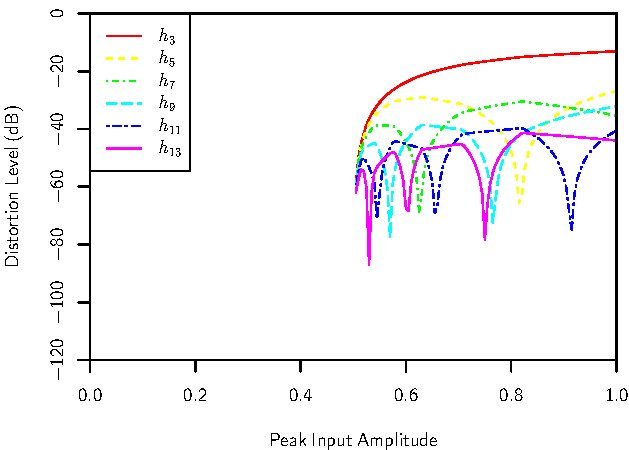
\includegraphics{chapter5/Images/HardClippingHarmonics.pdf}
				\caption{Individual harmonic distortion levels for Equation \ref{eq:SymmetricHardClipping}
					 with a threshold of 0.5.}
				\label{fig:HardClippingHarmonics}
			\end{figure}

			\begin{figure}[h!]
				\centering
				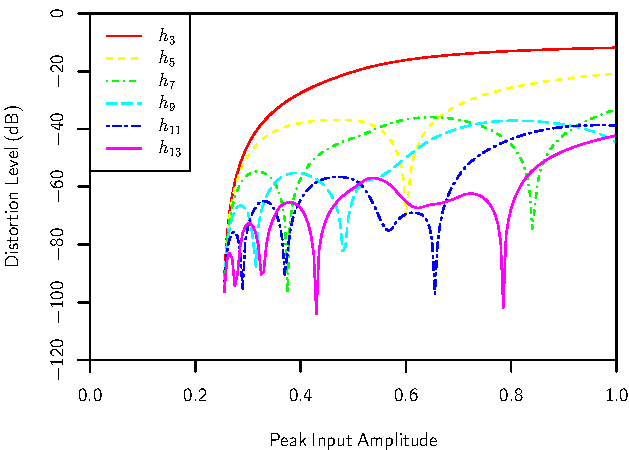
\includegraphics{chapter5/Images/SoftClippingHarmonics.pdf}
				\caption{Individual harmonic distortion levels for Equation \ref{eq:SymmetricSoftClipping}
					 with a threshold of 0.5.}
				\label{fig:SoftClippingHarmonics}
			\end{figure}

			The first thing to note is that new harmonic components are only introduced once the input amplitude
			extends out of the linear section of the characteristic curve. Once the input amplitude reaches a
			sufficient level harmonics are introduced but their amplitudes all vary independently. This
			behaviour can be improved on through the use of a different clipping function. Equation
			\ref{eq:SymmetricExponentialClipping} shows a function used to apply exponential clipping to a
			signal.
			
			\begin{equation}
				y[n] = \begin{cases}
					t\sgn(x[n]) & \text{if $\abs{x[n]} > t$} \\
					t\sgn(x[n]) \left(1 - \abs{\frac{x[n]}{t} - \sgn(x[n])}^{E} \right) &
						\text{otherwise}
				\end{cases}, \quad t \geq 0 \ \text{and} \ E > 1
				\label{eq:SymmetricExponentialClipping}
			\end{equation}

			Where $E$ is a second parameter called the exponent. One advantage of this clipper is that it has
			no linear section. This means that harmonics are generated for input signals of any amplitude.
			Another advantage is that the levels of the generated harmonics vary more uniformly with input
			amplitude as shown in Figure \ref{fig:ExponentialClippingHarmonics}.

			\begin{figure}[h!]
				\centering
				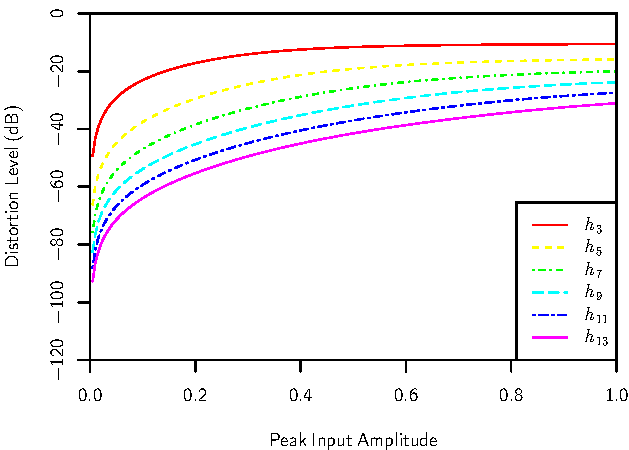
\includegraphics{chapter5/Images/ExponentialClippingHarmonics.pdf}
				\caption{Individual harmonic distortion levels for Equation
					 \ref{eq:SymmetricExponentialClipping} with a threshold of 0.5 and an 
				         exponent of 5.}
				\label{fig:ExponentialClippingHarmonics}
			\end{figure}

			The non-homogeneity of simple clipping systems can be counteracted by introducing gain stages
			either side of the clipping stage. The first gain stage scales the signal so that the clipping
			stage will always clip the same proportion of the signal. The second gain stage scales the signal
			back to the original input amplitude. Analogously the clipping function can be scaled so it
			always clips the same proportion of the signal, as done by \citet{deman2014adaptive}.

		\subsubsection*{Rectification}
			Rectifiers exhibit a less strict form of homogeneity; positive homogeneity. They satisfy Equation
			\ref{eq:homogeneity} only for non-negative values of $a$. For full wave rectification this can be
			summarised using Equation \ref{eq:FullWaveRectificationHomogeneity}. For negative values of $a$ the
			right hand side of the equation is the additive inverse of the left hand side. This has little
			effect on the use of a full wave rectifier as the output is always positive.

			\begin{equation}
				\abs{ax[n]} = a\abs{x[n]}, \quad a \geq 0
				\label{eq:FullWaveRectificationHomogeneity}
			\end{equation}

			Half wave rectification behaves slightly differently in that the sign of the gain applied to a
			signal before processing determines which parts of the signal are zeroed. If a negative gain is
			applied the positive portions of the original input are made negative and are therefore zeroed by
			the rectification. For simple signals, with similar negative and positive going portions, this is of
			no concern but for more complex signals the choice of which portions are zeroed may make a
			perceivable difference.

		\subsubsection*{Integrator}
			Integration is a homogeneous operation because of the distributive property of multiplication. The
			implementation give in Equation \ref{eq:Integrator} however only exhibits positive homogeneity due
			to the rectification of the signal prior to integration. The sign of the gain applied to the
			input signal also determines the points at which the output output signal is reset to zero.
			The signal is reset on positive going zero crossings but a negative gain before in the input
			reverses the direction of all zero crossings. Similarly to half wave rectification this may have
			audible effects depending on the nature of the input signal.

		\subsubsection*{Multiplier}
			Exponentiation is a non-homogeneous operation. Any gain applied to a signal prior to processing is
			also raised to the exponent, as shown in Equation \ref{eq:MultiplierHomogeneity}.

			\begin{equation}
				(ax[n])^{h} = a^{h}x[n]^{h}
				\label{eq:MultiplierHomogeneity}
			\end{equation}

			Unlike clipping algorithms there is no threshold parameter to change in response to the amplitude of
			the input signal. Gain stages can be added before and after the nonlinearity in order to make the
			system's response to different input amplitudes more uniform.

		\subsubsection*{SSBA}
			As with multipliers, SSBA is a non-homogeneous process. The amplitude envelope of the $h$\super{th}
			order automodulation is the amplitude envelope of the original signal raised to the power $h$. 

		\subsubsection*{IAP}
			The IAP method is homogeneous when used to generate odd order harmonics but is only positive
			homogeneous when used to generate even order harmonics. Equation \ref{eq:IAP} is easily shown to be
			positive homogeneous as application of a non-negative gain will alter only the amplitude of a signal
			leaving its phase information unchanged (Equation \ref{eq:IAPPositiveHomogeneity}).

			\begin{gather}
				\abs{ax_{a}[n]} = a\abs{x_{a}[n]} \nonumber \\
				\arg(ax_{a}[n]) = \arg(x_{a}[n]), \quad a \geq 0
				\label{eq:IAPPositiveHomogeneity}
			\end{gather}

			Application of a negative gain however changes the phase of the signal (Equation
			\ref{eq:NegativeGainPhase}).
						
			\begin{equation}
				\arg(ax_{a}[n]) = (\arg(x_{a}[n]) \mod 2\pi) - \pi, \quad a < 0
				\label{eq:NegativeGainPhase}
			\end{equation}

			When the phase is scaled to increase the frequency, the effects depend on the order of the harmonic
			being generated, $h$. The phase of the amplified signal, $ax_{a}[n]$, scaled by $h$ is $h\pi$
			radians less than that of the original signal, $x_{a}[n]$, scaled by the same factor (Equation
			\ref{eq:IAPOrderHomogeneity}).

			\begin{equation}
				h\arg(ax_{a}[n]) = h(\arg(x_{a}[n]) \mod 2\pi) - h\pi, \quad a < 0
				\label{eq:IAPOrderHomogeneity}
			\end{equation}

			The $-h\pi$ radian offset in phase introduced by the scaling means that the polarity of the output
			is changed depending on the parity of $h$. If the input signal to a harmonic excitation system using
			IAP is inverted the odd order harmonics generated will also be inverted while the even order ones
			will not. This could have dramatic timbral effects if the generated harmonics are being summed with
			other signals with the same frequency components.

		\subsubsection*{Spectral Stretching}
			The phase vocoder algorithm used for spectral stretching is a homogeneous system. When processing
			the signal in the frequency domain only the phase information is altered, leaving magnitude
			information unchanged. 

		\subsubsection*{Linear Time Variant Algorithms}
			The remaining algorithms (spectral replication using Equation \ref{eq:SpectralReplication}, spectral
			folding and STTR) are linear time variant systems. As such they all satisfy the principle of
			homogeneity.

%		\subsubsection*{Spectral Replication}
%			Spectral replication using Equation \ref{eq:SpectralReplication} linear time variant system, as such
%			it satisfies the condition of homogeneity.
%			
%		\subsubsection*{Spectral Folding}
%			Both downsampling and upsampling are homogeneous processes making spectral folding also
%			homogeneous.
%
%			\note
%			{
%				Formal proof?
%			}
%			
%		\subsubsection*{STTR}
%			STTR is a homogeneous process. As the samples in each frame are only multiplied by a constant window
%			and reversed in time none of the amplitude information in the signal is lost. 

	\subsection{Spectral Characteristics}
	\label{sec:ExcitationEvaluation-Comparison-SpectralCharacteristics}
		\subsubsection*{Static Nonlinearities}
			The spectral characteristics of a static nonlinearity depend on the function which describes its
			characteristic curve. If an odd function is used only odd order components will be produced, using
			an even function only even order components are generated. The symmetric clippers discussed
			previously are all described by odd functions. It is evident from the harmonic amplitude plots
			(Figures \ref{fig:HardClippingHarmonics}, \ref{fig:SoftClippingHarmonics} and
			\ref{fig:ExponentialClippingHarmonics}) that only odd order harmonics have been introduced to the
			signal. In order to generate even order harmonics these clipping function need to be made
			asymmetric. This is easily done by clipping negative and positive portions of the input signal at
			different thresholds. For example, Equation \ref{eq:SymmetricHardClipping} can be modified to allow
			for asymmetric clipping giving Equation \ref{eq:AsymmetricHardClipping}.
			
			\begin{equation}
				y[n] = \begin{cases}
					t_{+} & \text{if $x[n] > t_{+}$} \\
					t_{-} & \text{if $x[n] < t_{-}$} \\
					x[n] & \text{otherwise}
				\end{cases}, \quad t_{-} < t_{+}
				\label{eq:AsymmetricHardClipping}
			\end{equation}

			Where $t_{+}$ and $t_{-}$ are the clipping thresholds for positive and negative portions of the
			signal respectively. Figure \ref{fig:AsymmetricHardClippingHarmonics} shows the harmonic amplitude
			plot for Equation \ref{eq:AsymmetricHardClipping} with $t_{+} = 0.5$ and $t_{-} = -0.3$. While the
			system is still non-homogeneous, the introduced energy consists of both odd and even order
			distortion components.

			\begin{figure}[h!]
				\centering
				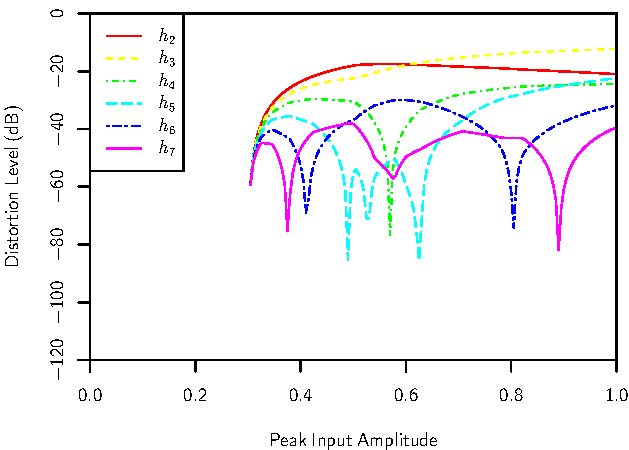
\includegraphics{chapter5/Images/AsymmetricHardClippingHarmonics.pdf}
				\caption{Individual harmonic distortion levels for Equation
					 \ref{eq:AsymmetricHardClipping} with thresholds of -0.3 and 0.5.}
				\label{fig:AsymmetricHardClippingHarmonics}
			\end{figure}

			The amplitudes of the generated harmonics will roll off at differing rates depending on the
			properties of the output signal. The spectrum will roll off at $6(n+1)$dB per octave when the
			$n$\super{th} derivative of the output signal is discontinuous \citep{kraght2000aliasing}.  Hard
			clippers introduce discontinuities to the first derivative of a signal and so will introduce
			harmonics whose amplitudes will roll off at 12dB per octave. Signals clipped by Equation
			\ref{eq:SymmetricSoftClipping} are continuous in the first derivative and so produce harmonics whose
			amplitudes roll off at a faster rate. This can be seen in Figure \ref{fig:ClippingSpectra}.

			\begin{figure}[h!]
				\centering
				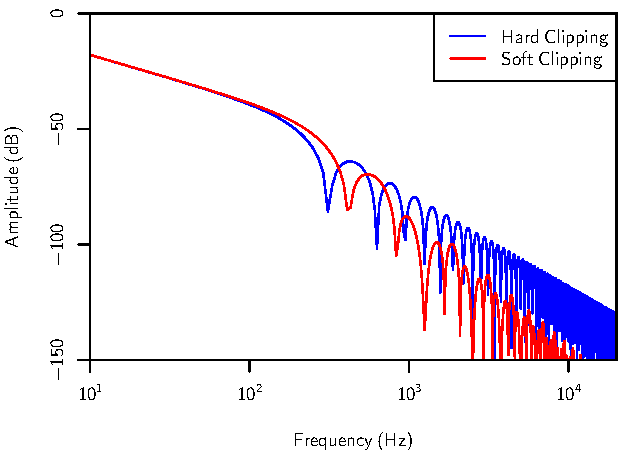
\includegraphics{chapter5/Images/ClippingSpectra.pdf}
				\caption{Spectra of sinusoids clipped using Equations \ref{eq:SymmetricHardClipping} and
			                 \ref{eq:SymmetricSoftClipping}.}
				\label{fig:ClippingSpectra}
			\end{figure}

			The large amount of spectral content introduced by static nonlinearities means they are particularly
			susceptible to aliasing. Through smoothing the characteristic curve of the nonlinearity (making the
			clipper `softer') the amplitudes of generated frequencies will roll of more quickly. With lower
			levels of high order distortion the amplitudes of any aliased components will be reduced. Aliasing
			can also be reduced by creating bandlimited approximations of a static nonlinearity's characteristic
			curve. A simple implementation of this is the Harmonic Mixer \citep{schattschneider1999discrete} in
			which low order polynomial expression approximating the desired characteristic curve is calculated.
			This could be achieved through linear regression as shown in Figure \ref{fig:ClippingApproximation}.
			The order of the polynomial used controls the maximum order of the distortion components,
			effectively eliminating those which would be aliased.

			\begin{figure}[h!]
				\centering
				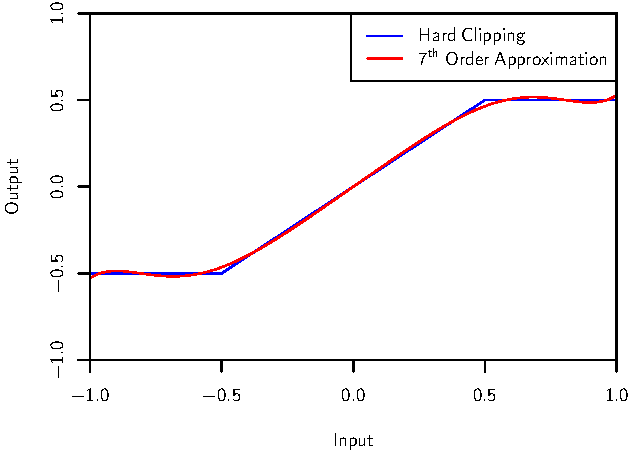
\includegraphics{chapter5/Images/ClippingApproximation.pdf}
				\caption{A 7\super{th} order approximation of hard clipping using linear regression.}
				\label{fig:ClippingApproximation}
			\end{figure}

			Generating characteristic curves in this way reduces the number of aliased frequencies at the cost
			of having to evaluate a more complex polynomial to calculate the output value for each sample. A
			similar approach is used by \citet{fernandez-cid2001distortion} who construct characteristic curves
			from Chebyshev polynomials in order to control the highest frequencies introduced.

			\citet{esqueda2015aliasing} propose a method for the reduction of aliasing in soft clipping systems,
			applying bandlimited hard clipping prior to the soft clipping. They show their method to reduced the
			level of aliased components when processing signals with $f_{0} < 3$kHz. While this method does not
			fully eliminate aliasing, it applies bandlimiting at the Nyquist ensuring that all orders of
			distortion which will not alias are left mostly unaffected. With a Harmonic Mixer one would have to
			select a distortion order based on the $f_{0}$ of the input signal to make the best use of the
			bandwidth allowed by the sampling frequency.

		\subsubsection*{Rectification}
			Full wave rectification can be considered as a static nonlinearity with an even characteristic
			curve, as such it only introduces even order distortion components. The Fourier series coefficients
			of a full wave rectified sine wave are shown in Equation \ref{eq:RectificationFourier}.

			\begin{gather}
				c_{n} = \frac{1}{2\pi} \int_{-\pi}^{\pi} \abs{sin(x)}e^{-inx} dx \nonumber \\
				c_{n} = \begin{cases}
					\frac{2}{\pi(1 - n^{2})} & \text{when $n$ is even} \\
					0 & \text{when $n$ is odd}
				\end{cases}
				\label{eq:RectificationFourier}
			\end{gather}

			This represents all even order harmonics rolling off at approximately 12dB per octave. As with
			other static nonlinearities, rectifiers are susceptible to aliasing. The relatively shallow roll
			off of the distortion components can lead to a considerable amount of energy present in the aliased
			components of the output signal. 

			The output from a half wave rectifier has the same spectrum as that of a full wave rectifier but
			with the content of the original signal included. This can easily be shown by considering how a half
			wave rectified signal can be constructed from the original signal and a full wave rectified signal.
			Where $x[n]$, $x_{f}[n]$ and $x_{h}[n]$ represent the original signal, full wave rectified and half
			waves rectified signals respectively, their relationship can be seen in Equation
			\ref{eq:RectificationRelationship}.

			\begin{equation}
				x_{h}[n] = \frac{1}{2} \left( x_{f}[n] + x[n] \right)
				\label{eq:RectificationRelationship}
			\end{equation}

		\subsubsection*{Integrator}
			Applying Equation \ref{eq:Integrator} to a sine wave produces a signal with Fourier series
			coefficients as shown in Equation \ref{eq:IntegratorFourier}.

			\begin{gather}
				c_{n} = \frac{kf_{s}}{2\pi} \left( \int_{0}^{\pi} (1 - cos(x))e^{-inx} dx +
							\int_{\pi}^{2\pi} (3 + cos(x))e^{-inx} dx \right) \nonumber \\
				c_{-1} = - \frac{2ikf_{s}}{\pi} \nonumber \\
				c_{0} = 2kf_{s} \nonumber \\
				c_{1} = \frac{2ikf_{s}}{\pi} \nonumber \\
				c_{n} = \frac{ikf_{s}}{2\pi} \left( \frac{4n^{2} + 2e^{-i\pi n} - 2}{n^{3} - n} \right)
				\label{eq:IntegratorFourier}
			\end{gather}

			This produces all harmonics with amplitudes rolling off at approximately 6dB per octave. This
			shallow roll of make integrators very useful when a large amount of new frequency content is
			desired. Due to the shallow roll off of the distortion component's amplitudes integrators are very
			prone to aliasing. While integrators are homogeneous, they are frequency dependant acting as low
			pass filters. Using the same integration constant a high frequency input signal will produce a lower
			amplitude output than a low frequency input. This does not affect the relatives amplitudes of
			frequencies in the output just the overall amplitude of the signal.

		\subsubsection*{Multiplier}
			Nonlinear processing using Equation \ref{eq:Multiplier}, in which the exponent is a positive
			integer, allows for control over the maximum order of distortion generated. The highest frequency
			present among those generated will be equal to the highest frequency in the input signal multiplied
			by the exponent. This facilitates more control over the bandwidth of the generated signal providing
			greater flexibility and minimisation of aliasing.

			If the exponent is allowed to take any positive value, control over the bandwidth of the output
			signal is lost. Non integer exponents cause higher orders of distortion to be generated. Figures
			\ref{fig:CubedSpectra} and \ref{fig:TwoAndAHalfSpectra} show the spectral effects of exponential
			static nonlinearities with integer and non-integer exponents. The input signal has a fundamental
			frequency of 1kHz and has energy in the first four harmonics.

			\begin{figure}[h!]
				\centering
				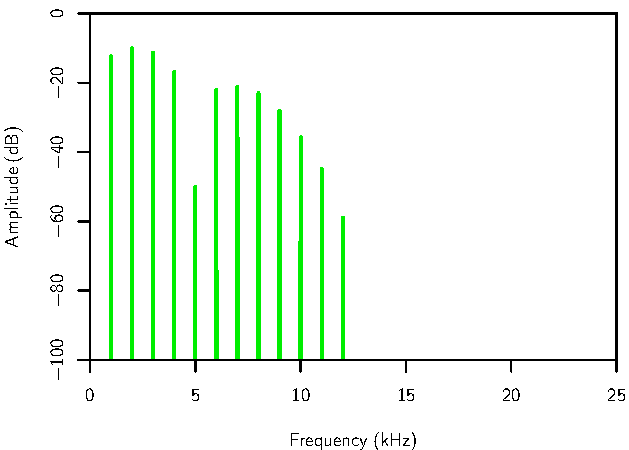
\includegraphics{chapter5/Images/CubedSpectra.pdf}
				\caption{The spectral effects of cubing a signal with energy in its first four harmonics.}
				\label{fig:CubedSpectra}
			\end{figure}

			\begin{figure}[h!]
				\centering
				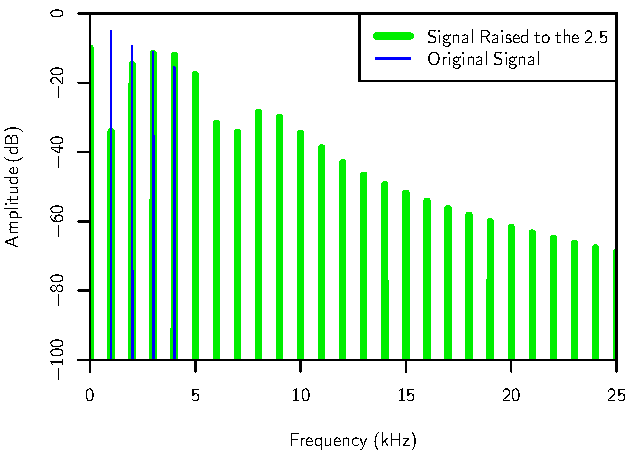
\includegraphics{chapter5/Images/RaisedToTwoAndAHalfSpectra.pdf}
				\caption{The spectral effects of raising a signal with energy in its first four harmonics
					 to the power 2.5.}
				\label{fig:TwoAndAHalfSpectra}
			\end{figure}

			The highest frequency component in the original signal is 4kHz. After cubing the signal the highest
			frequency is three times this (12kHz) as seen in Figure \ref{fig:CubedSpectra}. Figure
			\ref{fig:TwoAndAHalfSpectra} shows that when the exponent is 2.5 higher frequency components are
			introduced. The lowest frequency component in the output signal is not bound not matter what the
			exponent used is. For even exponents there will always be some 0Hz (DC offset) energy introduced.

		\subsubsection*{SSBA}
			SSBA extends the control provided by multipliers as it constrains the minimum frequency introduced
			as well as the highest. Using Equation \ref{eq:SSB} only the upper sideband (the sum frequencies)
			of the modulation is produced. The highest and lowest frequency components of the output are that
			of the input signal multiplied by the exponent. All other harmonic and intermodulation components
			created lie between these two frequencies. This can be seen in figure \ref{fig:SSBA3Spectra},
			which shows the results of applying $3$\super{rd} order SSBA to the signal used in Figures
			\ref{fig:CubedSpectra} and \ref{fig:TwoAndAHalfSpectra}. 			
			
			\begin{figure}[h!]
				\centering
				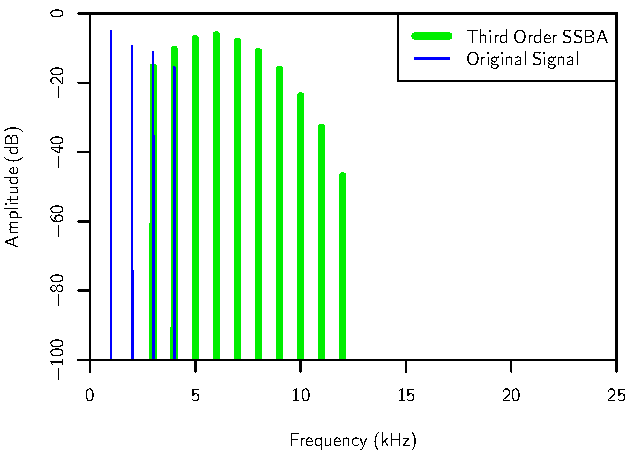
\includegraphics{chapter5/Images/SSBA3Spectra.pdf}
				\caption{The spectral effects of applying third order SSBA to a signal with energy in its 
				         first four harmonics.}
				\label{fig:SSBA3Spectra}
			\end{figure}

			If aliasing does occur it is possible for the aliased frequency to lie outside of this bandwidth.
			The amplitude of aliased frequencies can be greatly reduced through filtering. Applying a low pass
			filter with a cutoff frequency of $\frac{f_{s}}{2h}$ prior to processing will reduce the amplitude
			of any frequency content in the input which will cause aliasing when processed.

			The bounding of the frequencies in the output signal means that SSBA will produce a single harmonic
			if the input is a sinusoid. This is useful in situations when fine control is required over the
			content of the output spectrum. An output signal can be constructed through the generation of
			several individual harmonics.

		\subsubsection*{IAP}
			Like the SSBA method, if the input is sinusoidal the IAP method will generate a single harmonic. In
			contrast to the SSBA method, for more complex input signals the IAP method provides little control
			over the bandwidth of the output when the input has multiple frequency components. Figure
			\ref{fig:IAP3Spectra} shows the spectral effects of third order IAP processing on the same signal
			used when discussing previous algorithms.

			\begin{figure}[h!]
				\centering
				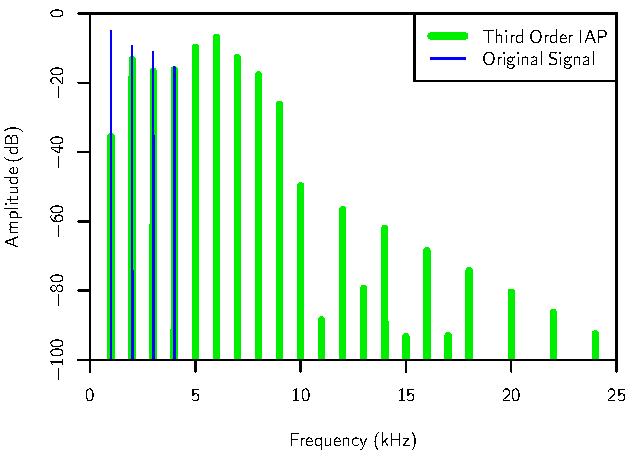
\includegraphics{chapter5/Images/IAP3Spectra.pdf}
				\caption{The spectral effects of applying third order IAP to a signal with energy in its 
				         first four harmonics.}
				\label{fig:IAP3Spectra}
			\end{figure}

			When multiple frequency components are present in the input signal, IAP processing produces energy
			at high order distortion components. As with previous algorithms, it may be necessary to upsample
			the signal before processing to avoid aliasing of these frequencies.

		\subsubsection*{Spectral Replication}
			In spectral replication each frequency component is shifted by the same amount, preserving the
			differences between them. This is useful for harmonic excitation of simple harmonically structured
			signals. Providing the spectrum is shifted by an integer multiple of the fundamental frequency any
			components at harmonic frequencies in the input will remain harmonic frequencies at the output. This
			process avoids the intermodulation distortion inherent to the systems discussed previously. 

			Due to every frequency component being shifted by an equal amount, the bandwidth of the output is
			equal to that of the input. This predictability allows for easier control of the output spectrum.
			It also provides a simple method for reduction of aliasing. The highest frequency in the output
			will be that of the input plus the shift frequency $f$. Applying a low pass filter, with a cutoff
			frequency of $f_{s} - f$Hz to the input will help minimise the amplitude of any aliased
			frequency components.

		\subsubsection*{Spectral Folding}
			Spectral folding with a factor $k$ results in the lowest $\frac{1}{k}$ of the input spectrum being
			repeated $k$ times in the output spectrum. Every second repetition is a mirror image of the
			original. This effect is shown in Figure \ref{fig:SpectralFolding}. 
			
			\begin{figure}[h!]
				\centering
				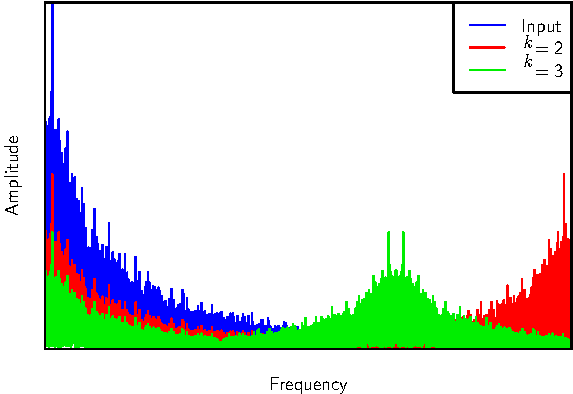
\includegraphics{chapter5/Images/SpectralFoldingSpectrum.pdf}
				\caption{The spectral characteristics of spectral folding.}
				\label{fig:SpectralFolding}
			\end{figure}

			The new frequencies introduced in the output depend on the sampling rate of the signal. Unless
			$\frac{f_{s}}{2k}$ is a harmonic of the input signal, there is little chance that the new
			frequencies will be harmonically related to the input.

			Other than changing the downsampling / upsampling factor, the user is given little control over the
			content of the output spectrum. The bandwidth of the output is not constricted, possibly taking up
			the entirety of the spectrum. Additional filtering is needed to shape the output spectrum as
			desired, increasing the overall complexity of the system.

		\subsubsection*{Spectral Stretching}
			An ideal spectral stretching system would produce the result shown in Figure
			\ref{fig:SpectralStretching}. All frequency components are scaled by the same factor preserving the
			frequency ratios between spectral components. For harmonically structured signals this has the
			effect of scaling the fundamental frequency, increasing the signals perceived pitch. The phase
			vocoder introduces some artefacts during its operation. The process of splitting the signal into
			frames causes spectral leakage; energy at a given frequency is spread across the nearby frequencies.
			In a signal which only has energy at harmonic frequencies, spectral stretching by an integer factor
			will produce some inharmonic content due to this effect. Spectral leakage can be minimised through
			the use of windowing functions such as the Hamming or Blackman-Harris windows.  Ignoring the effect
			of spectral leakage, the bandwidth of the output signal will be that of the input multiplied by the
			stretching factor. This allows for effective minimisation of aliasing as the signal can be low pass
			filtered before processing as done with single sideband automodulation.
		
		\subsubsection*{STTR}
			The spectral effects of STTR depends on the properties of the input signal and the window function
			and step size used. For simple sinusoidal inputs complex output spectra can be generated. For
			example, consider the spectral effects of STTR using the window function defined in Equation
			\ref{eq:STTRWindow} (shown in Figure \ref{fig:STTRWindow}). This window function exhibits constant
			overlap add for a step size of $\frac{L}{2}$. Figure \ref{fig:STTRSpectra} shows the output spectra
			of STTR, using this window with lengths of 1ms and 1.5ms, on a 1kHz sinusoid.

			\begin{equation}
				w[n] = \begin{cases}
					\cos \left( \frac{4\pi n}{3L} \right) & \text{if $\abs{n} \leq \frac{L}{4} $} \\
					1 - \cos \left( 2\pi \frac{2n - \sgn(n)L}{3L} \right) &
						\text{if $\frac{L}{4} < \abs{n} \leq \frac{L}{2}$} \\
					0 & \text{otherwise}
				\end{cases}
				\label{eq:STTRWindow}
			\end{equation}

			\begin{figure}[h!]
				\centering
				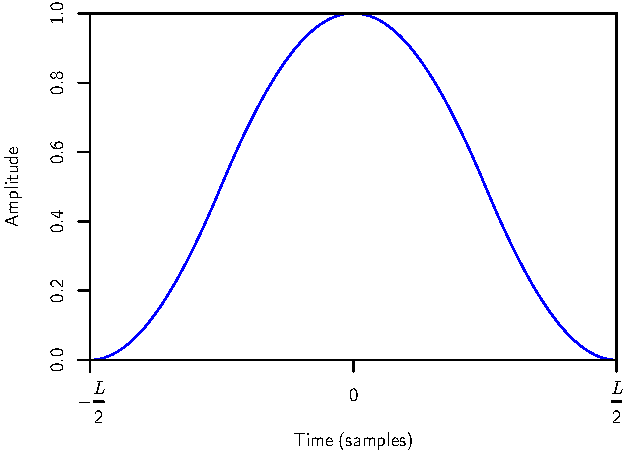
\includegraphics{chapter5/Images/STTRWindow.pdf}
				\caption{The window function defined in Equation \ref{eq:STTRWindow}.}
				\label{fig:STTRWindow}
			\end{figure}

			\begin{figure}[h!]
				\centering
				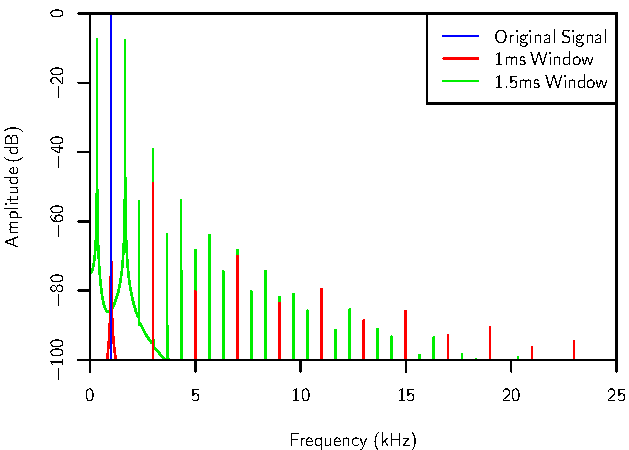
\includegraphics{chapter5/Images/STTRSpectra.pdf}
				\caption{The spectral effects of STTR using the window function defined in Equation
				         \ref{eq:STTRWindow}.}
				\label{fig:STTRSpectra}
			\end{figure}

			The complexity of the output spectrum depends on the relationship of the input frequency and the
			step size used for processing. If the period of the input signal is an integer multiple of the step
			size, it will remain unchanged by the processing. This is evidenced by the output spectrum for 1ms
			window shown in Figure \ref{fig:STTRSpectra}, only odd order harmonics are generated retaining the
			original period of the signal.

			The period of the output signal is equal to the least common multiple of the period of the input
			signal and the step size. This causes the period of a signal to be increased when the period of the
			input is not an integer multiple of the step size. The output spectrum for a 1.5ms window shows
			this. The period of the output becomes 3ms. The lowest frequency in this output is then
			approximately 333Hz.

			The exact frequencies of the partials in the output are discussed by \citet{kim2014shorttime}. In
			effect they are the intermodulation frequencies of the input frequency and the step frequency (1
			over the step size in seconds). The amplitudes of these partials are influenced by the Fourier
			transform of the window function used. This allows the spectral characteristics of the output to be
			loosely controlled through manipulation of the window function and step size. There is no upper
			bound on the frequency of the output so upsampling may need to be used to minimise aliasing.

	\subsection{Temporal Characteristics}
	\label{sec:ExcitationEvaluation-Comparison-TemporalCharacteristics}
		\subsubsection*{Static Nonlinearities}
			As static nonlinearities are memoryless they can not easily be used to control the temporal
			evolution of a signal. The amplitude of the characteristic curve for low amplitude samples can be
			manipulated to alter the attack and release times of signals. Increasing this amplitude will
			shortening attack and release times. As an extreme example consider the infinite peak clipper shown
			in Equation \ref{eq:InfinitePeakClipper}.

			\begin{equation}
				y[n] = \sgn(x[n])
				\label{eq:InfinitePeakClipper}
			\end{equation}
			
			Figure \ref{fig:InfinitePeakClipping} shows a signal, with attack and release sections, before and
			after infinite peak clipping. The original signal rises to its full amplitude over two cycles and
			falls back to silence over the same time. After infinite peak clipping the attack and release have
			become instantaneous.

			\begin{figure}[h!]
				\centering
				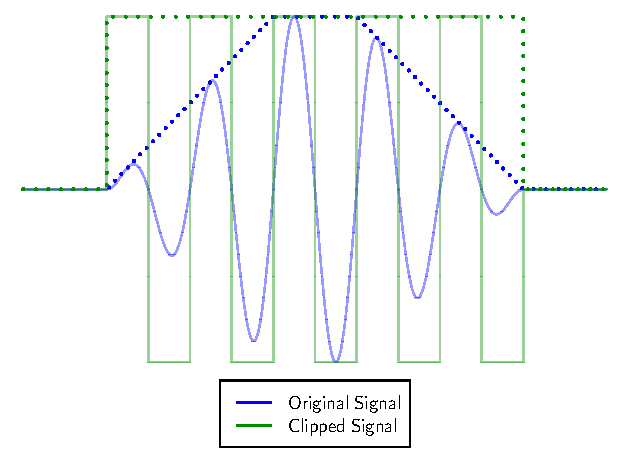
\includegraphics{chapter5/Images/InfinitePeakClipping.pdf}
				\caption{A graph showing a signal before and after infinite peak clipping.}
				\label{fig:InfinitePeakClipping}
			\end{figure}

			The exact change in attack / release time is dependant on both the characteristic curve of the
			nonlinearity and the existing temporal features of the input signal. For the infinite peak clipper
			all dynamic information in a signal is lost and all attack and release times are made instantaneous.
			Other static nonlinearities, such as soft peak clippers, have less predictable effects on temporal
			envelopes. 

		\subsubsection*{Rectification}
			Full wave rectifiers have no effect on the temporal characteristics of signals as the magnitude
			information of each sample is preserved. It is possible that a half wave rectifier could change the
			position of the onset / offset of a signal by a small amount. Considering a signal which starts with
			a negative displacement. This first section of the signal would be removed, moving the onset to the
			position of the first positive displacement occurs. This possible delay in onset is highly dependant
			on the input signal and will most likely be imperceptible.
			
		\subsubsection*{Integrator}
			Due to the inherent low pass filtering behaviour of integrators (see Section
			\ref{sec:ExcitationEvaluation-Comparison-SpectralCharacteristics}) the temporal properties of
			transient signals will be altered. Fast attacks times will be lengthened by the attenuation of their
			high frequency components. This prevents integrators being used for harmonic excitation in
			applications where it is essential that transients are preserved. 
			
		\subsubsection*{Multiplier}
			Exponential static nonlinearities have a dynamic compression / expansion effect. For exponents
			greater than 1 the dynamics of a signal are expanded, the amplitude difference between low and high
			amplitude portions of the signal is increased. For exponents less that 1 the opposite occurs,
			compressing the dynamics of the signal. Figure \ref{fig:ExponentiationTemporalEffects} show the
			effects this can have on the attack and release portions of signals.

			\begin{figure}[h!]
				\centering
				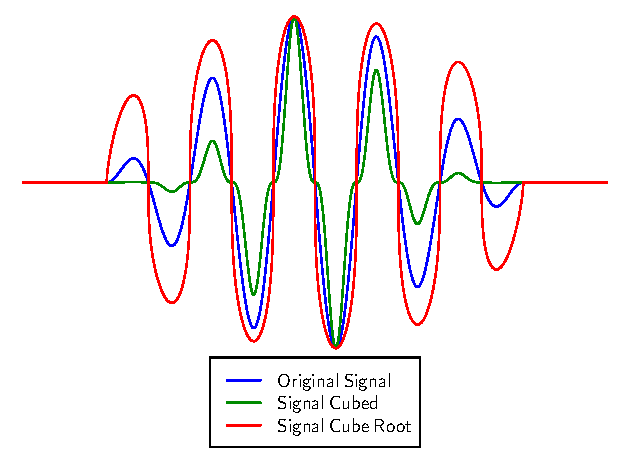
\includegraphics{chapter5/Images/ExponentiationTemporalEffects.pdf}
				\caption{The temporal effects of exponential static nonlinearities.}
				\label{fig:ExponentiationTemporalEffects}
			\end{figure}

			While the time taken for the signal to rise to or decay from maximum amplitude is not changed, the
			shape of the amplitude envelope during the attack and release portions is. Exponents greater than 1
			cause the amplitude to rise more slowly initially and then rapidly rise, while exponents less than
			one increase the initial gradient of the attack and then slowly rise to full amplitude. As with
			other static nonlinearities these effects are dependant on the input signal and are not predictable
			enough to give intuitive control.

		\subsubsection*{SSBA}
			SSBA has similar temporal effects to a multiplier using an exponent greater that 1. The signal
			undergoes dynamic expansion changing the shape of its attack and release envelopes as shown in
			Figure \ref{fig:SSBATemporalEffects}.

			\begin{figure}[h!]
				\centering
				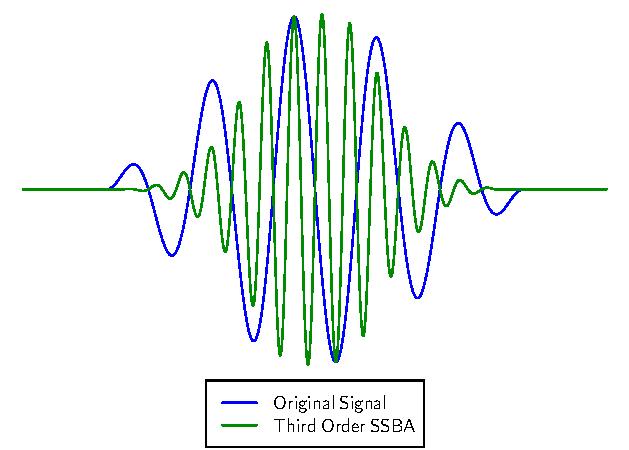
\includegraphics{chapter5/Images/SSBATemporalEffects.pdf}
				\caption{The temporal effects of SSBA.}
				\label{fig:SSBATemporalEffects}
			\end{figure}

			The restricted bandwidth of the SSBA technique's output is also apparent from this graph. The input
			is a sinusoid with a simple amplitude envelope. The output is a sinusoid with 3 times the frequency
			and an amplitude envelope equal to that of the input cubed. This is in contrast to the effect of
			the multiplier shown in Figure \ref{fig:ExponentiationTemporalEffects} where the output signal is
			no longer sinusoidal.

		\subsubsection*{IAP}
			The IAP system preserves the input signal's amplitude envelope. Due to this the temporal
			characteristics of signals are unaffected. This can be seen in Figure \ref{fig:IAPTemporalEffects},
			it is apparent that the frequency of the sinusoid has been altered and its amplitude envelope not.

			\begin{figure}[h!]
				\centering
				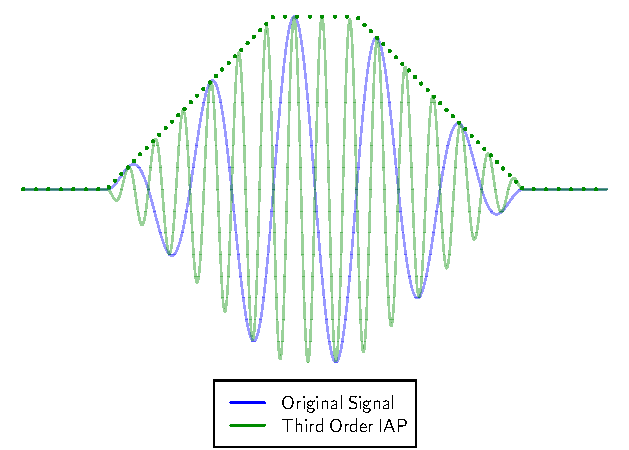
\includegraphics{chapter5/Images/IAPTemporalEffects.pdf}
				\caption{The temporal effects of IAP.}
				\label{fig:IAPTemporalEffects}
			\end{figure}
			
		\subsubsection*{Spectral Replication}
			As with IAP, spectral replication preserves the amplitude envelope of a signal, leaving its temporal
			characteristics unchanged.

		\subsubsection*{Spectral Folding}
			When using spectral folding, the low pass filter applied prior to the downsampling and upsampling
			process removes the high frequency content which contributes to transients in the signal. This has
			the effect of lengthening attack times similar to the effect seen in the integrator system. The
			degree, $k$, of spectral folding determines the cutoff frequency of the filter; higher values
			of $k$ removing more high frequency energy, causing longer attack times.

		\subsubsection*{Spectral Stretching}
			A simple phase vocoder implementation produces artefacts when processing transients in a signal.
			The phase correction stage before resynthesis can have the effect of softening the attack portion.
			The exact effect had on the transient is not able to be controlled as it depends on where the
			transient lies in the STFT frame. \citet{robel2003a} proposes a method to better process transients
			with a phase vocoder. An algorithm is used to detect the presence of transients in an STFT frame.
			The phase information is then processed differently depending on the position of the transient
			within the frame.

		\subsubsection*{STTR}
			Due to the time reversal STTR can have complicated effects on a signal's amplitude envelope.
			For instance, the attack and release portion of a sound may be switched. While possible, this is
			highly dependent on the window length, step size and content of the input frequency. Controlling
			these aspects for general input signals proves a very difficult task.

	\subsection{Flexibility}
	\label{sec:ExcitationEvaluation-Comparison-Flexibility}
		\subsubsection*{Static Nonlinearities}
			For musical signals static nonlinearities introduce a spectrally rich band of audio. The spectral
			content of which is highly dependent on that of the input signal. The bandwidth of the new set of
			frequencies can be easily controlled through filtering or through the techniques discussed for
			reducing aliasing. This allows for good performance in situations where energy needs to be added to
			a specific area of the spectrum. 

		\subsubsection*{Rectification}
			Rectifiers are useful when large amounts of even order distortion components are required. As with
			other static nonlinearities, the bandwidth of the newly introduced set of frequencies can be
			controlled through filtering to provide more flexibility. 

		\subsubsection*{Integrator}
			Integrators provide an efficient means to add wideband energy to the spectrum of a signal. All
			orders of distortion are generated making this new signal spectrally dense. The bandwidth of the
			new signal can easily be controlled through filtering improving the flexibility.

		\subsubsection*{Multiplier}
			Multipliers offer greater flexibility than the previously discussed excitation methods. Control
			over the orders of distortion introduced allows for finer shaping of a signal's spectrum. The
			output of several multipliers with different exponents can be summed in order to include multiple
			orders of distortion.

			Summing multiplier outputs in this way allows for approximation of other static
			nonlinearities. \note{Refer back to Section \ref{sec:ExcitationEvaluation-Comparison-Homogeneity}.}

		\subsubsection*{Spectral Folding}
			Spectral folding is an efficient method by which to create a dense output spectrum but has many
			downsides.

		\subsubsection*{STTR}
			STTR can be used, much like a static nonlinearity, as a method of generating wide bands of
			high order harmonics. Unlike static nonlinearities however it is possible to generate inharmonic
			partials for a sinusoidal input. The generation of these is dependent on properties of the input
			signal adding further complexity to predicting the effects for arbitrary input signals.

			\citet{kim2015harmonizing} suggest methods through which the output of STTR can be controlled in
			the implementation of a harmonising effect. This effect introduces new tones, at different
			musical intervals, depending on the input frequency. While this is useful as a compositional tool
			it does not provide the uniform response across input signals required for timbral control.

\section{Key Findings}
	\note
	{
		Conclude the chapter.
	}
